\documentclass{article}
\usepackage[utf8]{inputenc}
\usepackage{amsmath, amssymb, amsthm}
\usepackage[dvipsnames]{xcolor}
\usepackage{tikz}
\usetikzlibrary{calc}

\begin{document}

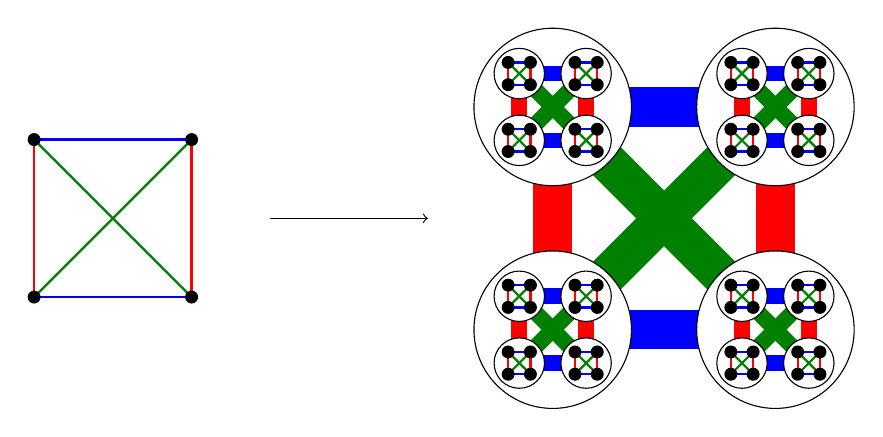
\begin{tikzpicture}

\draw[thick, red] (-8,1) -- (-8,-1);
\draw[thick, red] (-6,1) -- (-6,-1);
\draw[thick, blue] (-8,1) -- (-6,1);
\draw[thick, blue] (-8,-1) -- (-6,-1);
\draw[thick, Green] (-8,1) -- (-6,-1);
\draw[thick, Green] (-8,-1) -- (-6,1);
\draw[fill=black] (-8,1) circle (0.075);
\draw[fill=black] (-8,-1) circle (0.075);
\draw[fill=black] (-6,1) circle (0.075);
\draw[fill=black] (-6,-1) circle (0.075);

\draw[->] (-5,0) -- (-3,0);

\draw[thick, red] (45: 2) -- (-45: 2);
\draw[thick, red] (135: 2) -- (-135: 2);
\draw[thick, blue] (45: 2) -- (135: 2);
\draw[thick, blue] (-45: 2) -- (-135: 2);
\draw[thick, Green] (135: 2) -- (-45: 2);
\draw[thick, Green] (45: 2) -- (-135: 2);
 
\draw[line width=5mm, red] (45: 2) -- (-45: 2);
\draw[line width=5mm, red] (135: 2) -- (-135: 2);
\draw[line width=5mm, blue] (45: 2) -- (135: 2);
\draw[line width=5mm, blue] (-45: 2) -- (-135: 2);
\draw[line width=5mm, Green] (135: 2) -- (-45: 2);
\draw[line width=5mm, Green] (45: 2) -- (-135: 2);
 
\foreach \t in {0,...,3}{
        \draw[fill=white] (90*\t + 45: 2) circle (1);
    
      
        \draw[thick, red] ($(90*\t + 45: 2) + (45: 0.6)$) -- ($(90*\t + 45: 2) + (-45: 0.6)$);
        \draw[thick, red] ($(90*\t + 45: 2) + (135: 0.6)$) -- ($(90*\t + 45: 2) + (-135: 0.6)$);
        \draw[thick, blue] ($(90*\t + 45: 2) + (45: 0.6)$) -- ($(90*\t + 45: 2) + (135: 0.6)$);
        \draw[thick, blue] ($(90*\t + 45: 2) + (-45: 0.6)$) -- ($(90*\t + 45: 2) + (-135: 0.6)$);
        \draw[thick, Green] ($(90*\t + 45: 2) + (135: 0.6)$) -- ($(90*\t + 45: 2) + (-45: 0.6)$);
        \draw[thick, Green] ($(90*\t + 45: 2) + (45: 0.6)$) -- ($(90*\t + 45: 2) + (-135: 0.6)$);
        
        \draw[line width=2mm, red] ($(90*\t + 45: 2) + (45: 0.6)$) -- ($(90*\t + 45: 2) + (-45: 0.6)$);
        \draw[line width=2mm, red] ($(90*\t + 45: 2) + (135: 0.6)$) -- ($(90*\t + 45: 2) + (-135: 0.6)$);
        \draw[line width=2mm, blue] ($(90*\t + 45: 2) + (45: 0.6)$) -- ($(90*\t + 45: 2) + (135: 0.6)$);
        \draw[line width=2mm, blue] ($(90*\t + 45: 2) + (-45: 0.6)$) -- ($(90*\t + 45: 2) + (-135: 0.6)$);
        \draw[line width=2mm, Green] ($(90*\t + 45: 2) + (135: 0.6)$) -- ($(90*\t + 45: 2) + (-45: 0.6)$);
        \draw[line width=2mm, Green] ($(90*\t + 45: 2) + (45: 0.6)$) -- ($(90*\t + 45: 2) + (-135: 0.6)$);
        
        \foreach \s in {0,...,3}{
               
               \draw[fill=white] (90*\t + 45: 2) + (90*\s + 45: 0.6) circle (0.32);
               
               
               
            
               \draw[thick, red] ($(90*\t + 45: 2) + (90*\s + 45: 0.6) + (45: 0.2)$) -- ($(90*\t + 45: 2) + (90*\s + 45: 0.6) + (-45: 0.2)$);
               \draw[thick, red] ($(90*\t + 45: 2) + (90*\s + 45: 0.6) + (135: 0.2)$) -- ($(90*\t + 45: 2) + (90*\s + 45: 0.6) + (-135: 0.2)$);
               \draw[thick, blue] ($(90*\t + 45: 2) + (90*\s + 45: 0.6) + (45: 0.2)$) -- ($(90*\t + 45: 2) + (90*\s + 45: 0.6) + (135: 0.2)$);
               \draw[thick, blue] ($(90*\t + 45: 2) + (90*\s + 45: 0.6) + (-45: 0.2)$) -- ($(90*\t + 45: 2) + (90*\s + 45: 0.6) + (-135: 0.2)$);
               \draw[thick, Green] ($(90*\t + 45: 2) + (90*\s + 45: 0.6) + (45: 0.2)$) -- ($(90*\t + 45: 2) + (90*\s + 45: 0.6) + (-135: 0.2)$);
               \draw[thick, Green] ($(90*\t + 45: 2) + (90*\s + 45: 0.6) + (-45: 0.2)$) -- ($(90*\t + 45: 2) + (90*\s + 45: 0.6) + (135: 0.2)$);
               
               \foreach \q in {0,...,3}{
                       
                       \draw[fill=black] (90*\t + 45: 2) ++ (90*\s + 45: 0.6) + (90*\q + 45: 0.2) circle (0.075);
                       
               }
        }
}
\end{tikzpicture}

\end{document}